\documentclass{article}
\usepackage{graphicx} % Required for inserting images

\title{HMM for Speech Recognition}
\author{Anass Anhari Talib \\ Eric Muthomi Gitonga \\ Pol Vidal Miranda}


\date{May 28, 2025}

\begin{document}

\maketitle

\section{Introduction}
    
    This report presents our work on building a speech recognition system using \textbf{Hidden Markov Models (HMMs)}. Due to a widespread blackout in Spain during our academic term, we lost a full week of classes. Unfortunately, this affected our learning continuity, especially on advanced topics such as HMMs which were not fully covered before this assignment was given.
    
    Despite these difficulties, we approached this project with the aim of gaining practical experience on how to update probabilistic models for prediction. We relied on publicly available repositories and research work to implement and present a technical walk-through of HMM-based speech recognition.
    
\section{What is a Hidden Markov Model?}
    A Hidden Markov Model (HMM) is a statistical model used to represent systems that are stochastic (having a random probability distribution) and time-dependent, where the underlying states are hidden (unobservable) but can be inferred through observable outputs. It consists of:
    
    \begin{itemize}
        \item \textbf{States (S)}: Represent the hidden process.
        \item \textbf{Observations (O)}: Outputs generated by the hidden states.
        \item \textbf{Transition Probabilities (A)}: Probabilities of moving between states over time.
        \item \textbf{Emission Probabilities (B)}: Probabilities of an observation being generated from a state.
        \item \textbf{Initial State Probabilities} ($\pi$): Probabilities of starting in each state.
        \item \textbf{State Space (S)}: The set of all possible hidden states.
        \item \textbf{Observation Space (O)}: The set of all possible observations.
    \end{itemize}
     
    The idea is to learn the parameters of this model from labeled audio data. Once trained, given a new sequence of audio features, we can use the model to determine which word (or phoneme sequence) was likely spoken. HMMs are widely used in applications like speech recognition, bioinformatics, and sequence prediction, where temporal or sequential data plays a key role.
    
\section{Step-by-Step Pipeline}
    
    The notebook we followed implements an end-to-end system for speech recognition using HMMs. Below, we summarize and expand each step we took.
    
\begin{enumerate}
        \item \textbf{Audio Input and Visualization}
        
    We began by reading '.wav' files using the \texttt{scipy.io.wavfile} module. This gives us both:
    \begin{itemize}
        \item The \textbf{sampling frequency} (e.g., 16,000 Hz).
        \item The raw \textbf{audio waveform}, which is just a sequence of numbers representing sound pressure.
    \end{itemize}
    
    We plotted the audio waveform to visualize how sound varies over time. This helps us understand the data before processing it. The resulting files were stereo audio of shape (stereo: (n$\_$samples, 2)).

    \begin{figure}[h!]
        \centering
        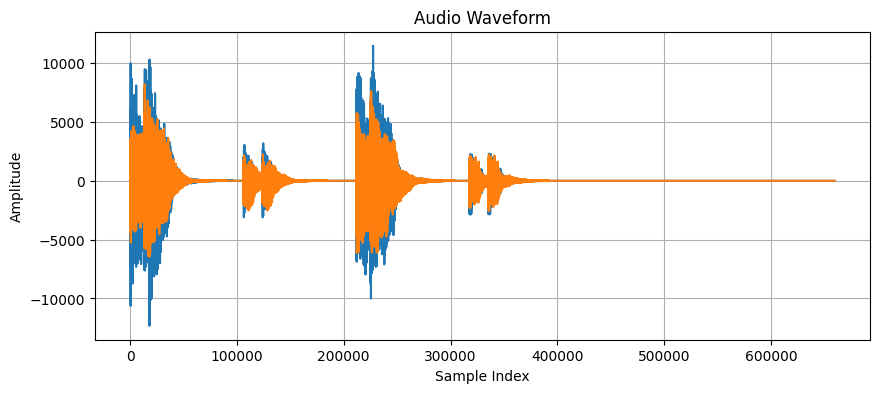
\includegraphics[width=1.0\linewidth]{stereo.png}
        \caption{Stereo Audio output}
        \label{fig:enter-label}
    \end{figure}
    
    \item \textbf{Preprocessing and Normalization}
    
    \begin{itemize}
    
        \item \textbf{Normalization}: The audio signal is scaled to a range between `-1` and `1` by dividing by the maximum possible value or the maximum absolute value of the signal.
        
        \item \textbf{Root Mean Square (RMS) Scaling}: The RMS of the signal is calculated to represent its energy, and the signal is scaled to a target RMS value (e.g., 0.1) to ensure consistent loudness across all audio samples.
        
        \item \textbf{Truncation}: Optionally limits the audio to the first 30 samples, likely for testing or computational efficiency.
    \end{itemize}
    
    \item \textbf{Feature Extraction – MFCCs}

    Rather than using the raw waveform (which has thousands of values), we extracted features called \textbf{MFCCs} (Mel-Frequency Cepstral Coefficients).
    
    MFCCs are compact numerical representations of the speech signal that:
    \begin{itemize}
        \item Reduce the dimensionality of the data while retaining perceptually important information. 
        \item Are commonly used in speech and audio classification tasks.
    \end{itemize}
    
    The first 13 MFCCs (Mel-Frequency Cepstral Coefficients) are extracted from an audio signal to represent its spectral characteristics. 
    
    \begin{table}[h!]
        \centering
        \begin{tabular}{|c|l|}
            \hline
            \textbf{MFCC Index} & \textbf{Interpretation} \\
            \hline
            \textbf{MFCC 1}  & Represents the overall energy of the signal (similar to loudness). \\
            \textbf{MFCC 2}  & Captures broad spectral shape, related to the formant structure. \\
            \textbf{MFCC 3}  & Represents finer details of the first formant (F1). \\
            \textbf{MFCC 4}  & Captures information about the second formant (F2). \\
            \textbf{MFCC 5}  & Describes additional spectral shape variations. \\
            \textbf{MFCC 6}  & Captures higher frequency spectral characteristics. \\
            \textbf{MFCC 7}  & Contains mid-range frequency variations. \\
            \textbf{MFCC 8}  & Represents slightly higher frequency spectral shape. \\
            \textbf{MFCC 9}  & Captures subtle frequency variations important for distinguishing phonemes. \\
            \textbf{MFCC 10} & Represents rapid spectral transitions. \\
            \textbf{MFCC 11} & Captures fine-grained variations in spectral features. \\
            \textbf{MFCC 12} & Sensitive to high-frequency spectral changes. \\
            \textbf{MFCC 13} & Represents the finest details of the speech signal. \\
            \hline
        \end{tabular}
        \caption{MFCC Index and Interpretation}
        \label{tab:mfcc}
    \end{table}
    
    Note that MFCC 1 is different from the others because it represents energy rather than spectral shape.
    MFCCs 2-13 primarily describe the shape of the spectral envelope, which helps in differentiating phonemes in speech recognition and identifying different sounds.
    
    \textbf{Why Consider Only few Out of 39 Features in MFCC?}
    
    MFCCs are commonly used in speech and sound processing. Typically, 39 features are extracted per frame, but many applications reduce this to only 13 – 15 features. 

    \item \textbf{Data Augmentation}

    To improve model robustness and reduce overfitting, we artificially created more audio data using:
    \begin{itemize}
        \item \textbf{Pitch shifting} (making audio sound higher or lower).
        \item \textbf{Speed changes} (making speech faster or slower).
        \item \textbf{Time stretching} (changing duration without altering pitch).
    \end{itemize}
    
    This helped the model generalize better to different voices and recording conditions.
    
    \item \textbf{HMM Training per Word}
    
    We trained a separate HMM for each word in the dataset. That means:
    \begin{itemize}
        \item All audio examples for the word “yes” were used to train one HMM.
        \item All examples for “no” trained a different HMM.
    \end{itemize}
    
    Each HMM learned the statistical structure (patterns) of the audio features representing its corresponding word.

    \item \textbf{Classification via Scoring}

    Once all HMMs were trained, we used them to classify new audio samples:
    \begin{itemize}
        \item For each sample, we calculated the \textbf{log-likelihood score} under every HMM.
        \item The model that gave the highest score was assumed to be the predicted class.
    \end{itemize}
    
    To improve this further, these scores were used as features for a simple \textbf{logistic regression classifier}, providing a final decision.

\end{enumerate}    

\section{Results and Evaluation}
    
    We evaluated the system using:
    \begin{itemize}
        \item \textbf{Confusion matrices}:  Shows whether the model's predictions converged or diverged from the actual true labels.
        The model showed promising results. However, this was not void of some false positives (FP) and false negatives (FN). The model on multiple occasions predicted 'kiwi' as being an 'apple' and vice versa, which showed the limitations of the model.

        \begin{figure}[h!]
            \centering
            \includegraphics[width=0.7\linewidth]{confusion.png}
            \caption{Confusion Matrix for audio files}
            \label{fig:enter-label}
        \end{figure}
        
        \item \textbf{Accuracy scores}: The model got an acceptable accuracy score of 0.64.
    \end{itemize}
    
    Despite the complexity of speech recognition and our short timeline, the model showed encouraging results and worked reliably for basic commands.
    
    \section*{Challenges of HMM models}
     
    HMM often struggles to classify different sounds using a single model due to several key limitations:
    
    \begin{enumerate}
        \item \textbf{HMM Assumes Stationarity and Markovian Properties}
        \begin{itemize}
            \item HMM assumes that the state transitions depend only on the previous state, which is a \textbf{first-order Markov assumption}.
            \item However, sound signals often have \textbf{long-term dependencies} and require context beyond the previous state.
        \end{itemize}
    
        \item \textbf{HMM is Generative, Not Discriminative}
        \begin{itemize}
            \item HMM is a \textbf{generative model}, meaning it estimates the \textbf{joint probability} of observations and hidden states.
            \item Classification tasks are better suited for \textbf{discriminative models} like Deep Neural Networks (DNNs).
        \end{itemize}
    
        \item \textbf{Limited Feature Representation}
        \begin{itemize}
            \item HMM uses simple \textbf{Gaussian Mixture Models (GMMs)} or discrete emission probabilities for feature modeling.
            \item This representation is often inadequate for complex sound patterns where deep learning models such as CNNs, BiLSTMs can extract \textbf{better hierarchical features}.
        \end{itemize}
    
        \item \textbf{Noise and Overlapping Sounds}
        \begin{itemize}
            \item HMMs assume \textbf{clean and structured sequences}, making them \textbf{prone to misclassification} in real-world noisy environments.
        \end{itemize}
    \end{enumerate}

    \section*{Application Scope}
    \begin{itemize}
        \item For traditional tasks: HMM, GMM, and Kalman Filters are reliable.
        \item For modern approaches: RNNs, Transformers, and CNNs offer greater flexibility and accuracy but require more data and computation.
        \item Emerging trends: Models like WaveNet and Transformers are setting new standards in speech and audio processing.
    \end{itemize}
    
\section*{Reflections and Conclusion}

This project was a valuable learning experience. Working under the pressure of a lost week due to a national power blackout — with reduced access to classes, guidance, and time — was extremely challenging.

We did not fully understand HMMs at the start. The theory is complex and we lacked time to deeply study the math behind it. However, by following a structured and practical approach, we were able to build a working system and, in the process, gained a meaningful understanding of how HMMs apply real-world audio for speech recognition.

\subsection*{Things We Learned}

\begin{itemize}
    \item The importance of preprocessing and normalization in audio tasks.
    \item How MFCCs transform raw sound into meaningful features.
    \item The intuition of HMMs — modeling sequences of data with state transitions.
    \item That data augmentation is key for performance, even in simple models.
\end{itemize}

\subsection*{Final Thoughts}

This report does not present a perfect or deeply academic solution, but rather a sincere and resilient attempt by students facing real obstacles. We hope our work reflects a spirit of effort, learning, and adaptation.

\end{document}
